\documentclass[a4paper,]{article}
\usepackage[left=2.5cm,top=2.5cm,right=2.5cm,bottom=3cm]{geometry} 
\usepackage[utf8]{inputenc}
\usepackage{graphicx} % Required for inserting images
\usepackage[table,xcdraw]{xcolor}
\usepackage{lipsum} % for dummy text
\usepackage{mathdots} % para el comando \iddots
\usepackage{mathrsfs} % para formato de letra
\usepackage{marvosym}
\usepackage{amsmath}
\usepackage{amsfonts}
\usepackage{amssymb}
\usepackage{listings}
\usepackage{caption}
\usepackage{float}


\title{\textbf{HW2: Introduction to Financial Engineering} \\ Time series}
\author{Miguel Angel Aguilo Gonzalez, 1699413 \\ Judit de Paz Ramírez, 1570590 \\ Laia Mòdol Rodríguez, 1565282 \\ Elena Rubio Zabala, 1699049 \\ Guillem Tutusaus Alcaraz, 1533701 } 
\date{Octubre 2023}

\begin{document}

\maketitle
\newpage

\section*{Ejercicio 1}
Queremos hacer un análisis de la serie temporal sobre los datos de 91-day Treasury Bill Rate. Vamos a empezar haciendo distintos gráficos de la serie temporal para saber cuál es su comportamiento. \\

Como queremos saber si la serie es estacionaria o no, hacemos tres tipos de gráficos:
\begin{figure}[H]
    \centering
    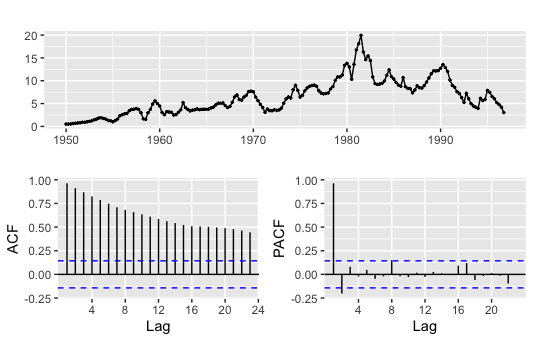
\includegraphics[width=0.5\linewidth]{1a.png}
\end{figure}
Lo primero que se puede ver en el primer gráfico es que, en promedio, la tasa aumenta hasta 1970. A partir de ahí, observamos como la tasa se reduce a la mitad para luego crecer de nuevo. Vemos también que durante diez años la tasa crece hasta llegar a su máximo en 1982, una vez alcanzado éste decrece de nuevo.\\

Dados estos largos períodos monótonos, podríamos pensar que esta serie no es estacionaria. Para poder confirmar estas suposiciones nos fijamos en el gráfico ACF dónde vemos que la función de la serie temporal disminuye de manera lenta con \textit{lags} muy alejados de cero. Esto es una clara señal de que la serie no es estacionaria. \\

Una vez hecho el estudio gráfico, procedemos a hacer el estudio numérico. \\

Veamos si la serie es estacionaria o no utilizando una prueba de la raíz unitaria. Existen dos pruebas principales de la raíz unitaria:
\begin{itemize}
    \item Dickey-Fuller: esta prueba busca determinar la existencia o no de raíces unitarias en una serie temporal. La hipótesis nula de esta prueba es que existe una raíz unitaria en la serie y la alternativa es que la serie es estacionaria. Los resultados incluyen estadísticas de la prueba, el valor p. Sabemos que si este valor es menor que 0,05, podemos rechazar la hipótesis nula.
    \item KPPS: esta prueba determina si una serie temporal es estacionaria alrededor de una tendencia media o lineal, o si no es estacionaria debido a una raíz unitaria. La hipótesis nula de la prueba es que los datos son estacionarios y la hipótesis alternativa es que no lo son. Nos fijaremos en el p-valor para decidir si nos quedamos o rechazamos la hipótesis nula.
\end{itemize}
Haciendo las dos pruebas obtenemos los siguientes p-valores:
\begin{table}[H]
\centering
\begin{tabular}{|l|l|l|}
\hline
\rowcolor[HTML]{C0C0C0} 
{\color[HTML]{000000} Prueba}         & {\color[HTML]{000000} p-valor} & {\color[HTML]{000000} Resultado} \\ \hline
\cellcolor[HTML]{EFEFEF}Dickey-Fuller & 0.6075                         & No estacionaria                  \\ \hline
\cellcolor[HTML]{EFEFEF}KPPS          & \textless{}0.01                & No estacionaria                  \\ \hline
\end{tabular}
\end{table}
Como podemos ver en la tabla, ambos p-valores son menores que el valor significativo (0,05), por lo tanto, podemos concluir que la serie con la que estamos trabajando no es estacionaria. \\

De todas maneras, no estamos del todo seguro de que la serie no sea estacionaria, así que volvemos a hacer el mismo estudio con la serie transformada. Volvemos a hacer los mismos tres gráficos:
\begin{figure}[H]
    \centering
    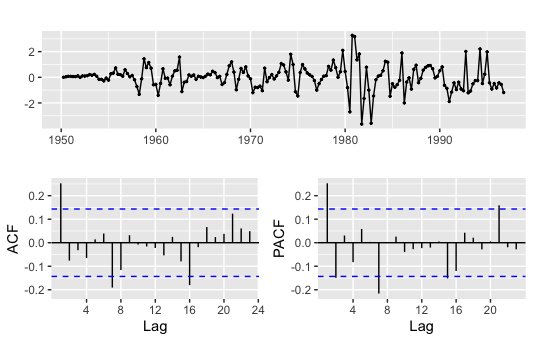
\includegraphics[width=0.5\linewidth]{1aa.png}
\end{figure}
En el primer gráfico, en particular en la primera mitad, se puede ver una aparente reversión de la media, por lo que podría ser probable que la serie temporal fuese estacionaria. Podemos observar también que la volatilidad aumenta en el periodo de 1950 a 1965, desde 1965 a 1980 se reajusta en el medio y desde 1980 parece permanecer constante. \\

Si nos fijamos en el gráfico ACF, vemos que éste disminuye a cero de manera rápida y, después del primer \textit{lag}, la mayoría de los valores no son significativos porque están dentro del nivel de significancia. Podemos suponer que la serie temporal transformada es estacionaria.\\

Para afirmar o negar nuestra hipótesis hacemos de nuevo las dos pruebas, en este caso obtenemos los siguientes p-valores:
\begin{table}[H]
\centering
\begin{tabular}{|l|l|l|}
\hline
\rowcolor[HTML]{C0C0C0} 
{\color[HTML]{000000} Prueba}         & {\color[HTML]{000000} p-valor} & {\color[HTML]{000000} Resultado} \\ \hline
\cellcolor[HTML]{EFEFEF}Dickey-Fuller & \textless{}0.01                & Estacionaria                     \\ \hline
\cellcolor[HTML]{EFEFEF}KPPS          & \textless{}0.01                & No estacionaria                  \\ \hline
\end{tabular}
\end{table}
En esta tabla vemos que cada prueba nos da un resultado diferente. La prueba Dickey-Fuller nos dice que la serie temporal es estacionaria, en cambio, la prueba KPPS nos dice que no lo es. Esto significa que la serie temporal es estacionaria en términos de tendencia.\\

Finalmente sabemos que una secuencia de variables aleatorias es heterocedástica si la variabilidad de la perturbación aleatoria es diferente entre los elementos del vector. En este caso vemos que la varianza de la serie transformada es considerablemente mayor a principios de 1980 que al comienzo de la serie temporal y que muestra agrupaciones de volatilidad. Todo esto nos indica que necesitaremos un modelo $GARCH$ que se ajuste a nuestros datos. \\

Tal y como hemos dicho, necesitamos un modelo que se ajuste a nuestros datos. De tal manera ajustaremos ahora a nuestra serie transformada un modelo $ARMA(1,0)/GARCH(1,0)$. Usando la función \texttt{garchFit} en R obtenemos la siguiente estimación de los parámetros del modelo:
$$\hat{\mu}=0.08349652 \hspace{1cm} \hat{\phi}=0.24163450 \hspace{1cm} \hat{\omega}=0.33815662 \hspace{1cm} \hat{\alpha}=0.83482811.$$
Esta misma función nos proporciona también los diferentes p-valores de los parámetros bajo las siguientes hipótesis; la hipótesis nula nos dice que el valor de los parámetros es igual a cero. La hipótesis alternativa nos dice que el valor de los parámetros es diferente a cero y por lo tanto, éstos son significativos. La siguiente tabla muestra los diferentes p-valores obtenidos:
\begin{table}[H]
\centering
\begin{tabular}{|
>{\columncolor[HTML]{EFEFEF}}c |c|c|}
\hline
\cellcolor[HTML]{C0C0C0}{\color[HTML]{000000} Parámetro} & \cellcolor[HTML]{C0C0C0}{\color[HTML]{000000} p-valor} & \cellcolor[HTML]{C0C0C0}{\color[HTML]{000000} Resultado} \\ \hline
$\hat{\mu}$                                              & $1.213955\cdot 10^{-1}$                                & Significativo                                            \\ \hline
$\hat{\phi}$                                             & $9.024598\cdot 10^{-4}$                                & Significativo                                            \\ \hline
$\hat{\omega}$                                           & $3.729535\cdot 10^{-8}$                                & Significativo                                            \\ \hline
$\hat{\alpha}$                                           & $5.899382\cdot 10^{-4}$                                & Significativo                                            \\ \hline
\end{tabular}
\end{table}

Dado que todos los valores anteriores son menores que el nivel de significancia impuesto, 0.05, rechazamos la hipótesis nula y aceptamos que los parámetros del modelo son estadísticamente significativos.\\

Trabajamos ahora con los residuos de la serie temporal diferenciada. Éstos tienen el siguiente gráfico:
\begin{figure}[H]
    \centering
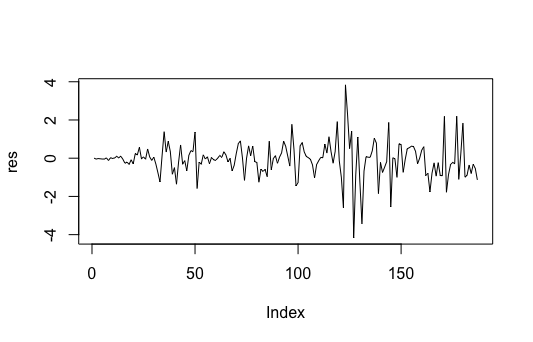
\includegraphics[width=0.5\linewidth]{1c.png}
\end{figure}
Podemos ver que el gráfico muestra una reversión a la media, tal y como era de esperar. Vemos también que la volatilidad parece ser menor en la primera mitad que en la segunda. A pesar de que los cambios en la volatilidad no son grandes, observamos que los residuos no parecen seguir una distribución \textit{white noise}.\\

Para comprobar este último hecho, haremos un par de gráficos más que nos darán más información de nuestro modelo. \\

Primero hacemos el gráfico ACF de los residuos, sabemos que los residuos se caracterizan por una falta de independencia, aunque no están correlacionados entre sí, porque su varianza condicional depende del tiempo. El gráfico ACF nos da una indicación de cómo modelar los residuos del conjunto de datos.
\begin{figure}[H]
    \centering
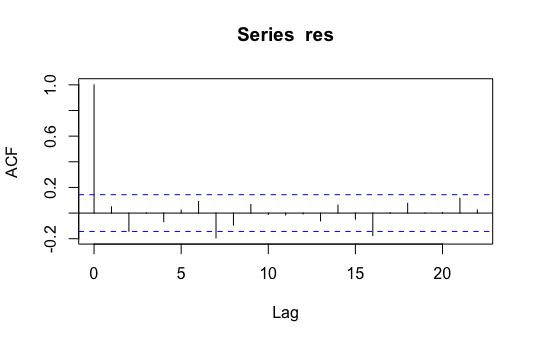
\includegraphics[width=0.5\linewidth]{1cacfres.png}
\end{figure}
Podemos ver en primer lugar que, en la parte $ARMA$ no hay ningún \textit{lag} que sobrepase el nivel de significancia de manera significativa y por lo tanto, no podemos suponer que los residuos no estén autocorrelacionados y no es posible ajustar los residuos con el método $ARMA$. \\

Para continuar, estudiaremos si hay una parte $GARCH$ mediante el gráfico ACF de los residuos al cuadrado.
\begin{figure}[H]
    \centering
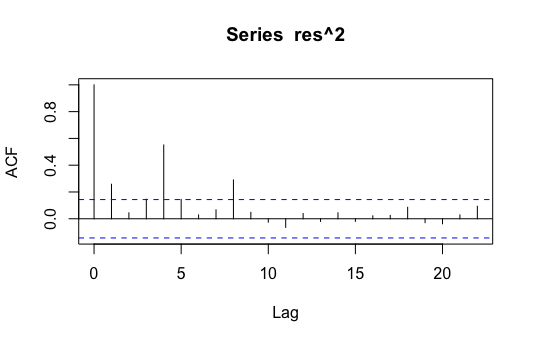
\includegraphics[width=0.5\linewidth]{1cacfrees^2.png}   
\end{figure}
En el gráfico se puede ver que hay tres \textit{lags} que sobrepasan el umbral de confianza, este hecho nos indica una autocorrelación nula. Se podría deducir que el modelo $ARMA(1,0)/GARCH(1,0)$ no es un modelo adecuado para nuestros datos. Para explicar correctamente el comportamiento de los residuos estudiaremos ahora los residuos estandarizados.\\

Hacemos el gráfico ACF de los residuos estandarizados al cuadrado:
\begin{figure}[H]
    \centering 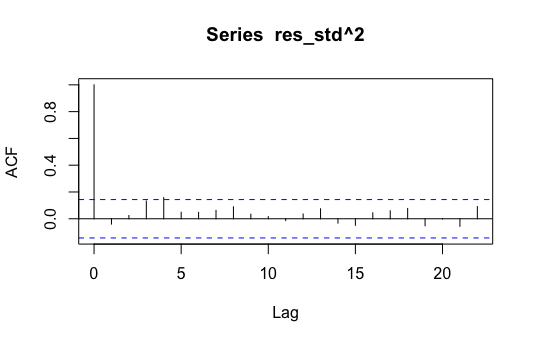
\includegraphics[width=0.5\linewidth]{resstd^2.png}
\end{figure}
Podemos ver en él que todos los valores se encuentran dentro del nivel de significancia cero y por lo tanto, se observa que los residuos estandarizados al cuadrado no están correlacionados. Como los valores se encuentran dentro del nivel de significancia, entonces podemos decir que la varianza es constante y por lo tanto, este modelo ajusta bien. \\

Finalmente estudiamos el comportamiento del gráfico de los residuos estandarizados a lo largo del tiempo.
\begin{figure}[H]
    \centering
    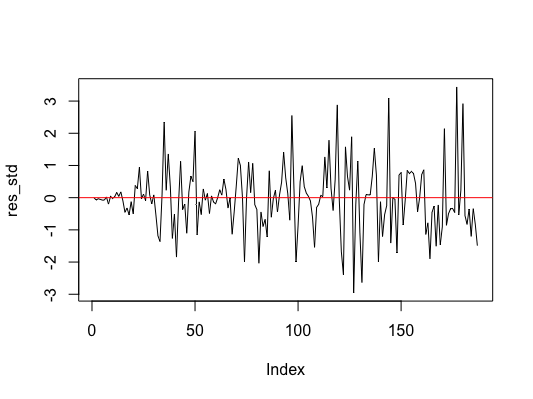
\includegraphics[width=0.5\linewidth]{resstd.png}
   % 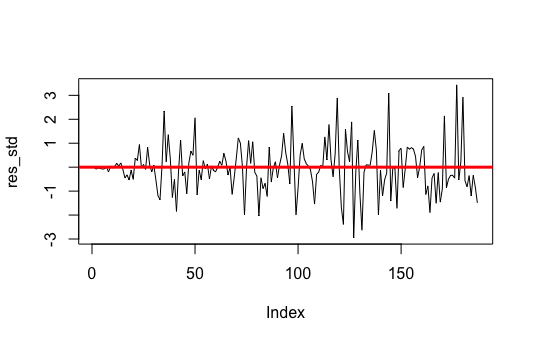
\includegraphics[width=0.5\linewidth]{resstdlinered.png}  
\end{figure}
Podemos observar que la varianza de los residuos parece aumentar con el tiempo, lo que nos puede llevar a pensar que la varianza no es constante y por lo tanto, no son variables independientes. \\

Para finalizar el estudio de los datos volvemos a transformar la serie temporal usando logaritmos. Queremos ajustar un modelo $ARMA/GARCH$ a la serie transformada. De nuevo hacemos el gráfico de la serie, el gráfico ACF y el gráfico PACF. 
\begin{figure}[H]
    \centering
    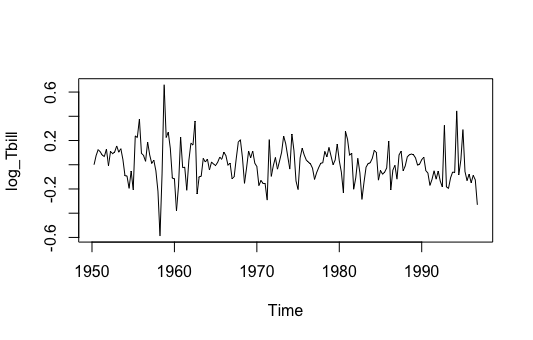
\includegraphics[width=0.5\linewidth]{plotlogtbill.png}
\end{figure}
\begin{figure}[H]
    \centering
     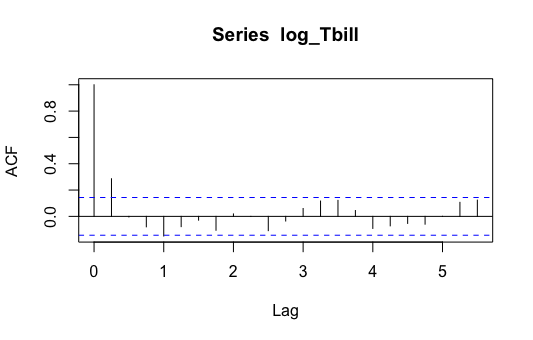
\includegraphics[width=0.4\linewidth]{acflogtbill.png}
    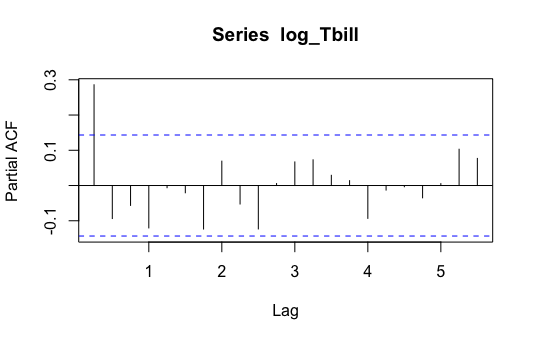
\includegraphics[width=0.4\linewidth]{pacflogtbill.png}
\end{figure}
Podemos ver que, gracias al logaritmo, la varianza parece más estabilizada sin muchas fluctuaciones. La transformación que hemos realizado nos da que la autocorrelación de los residuos es nula, tal y como podemos ver en el gráfico ACF. \\

Además, observando los gráficos ACF y PACF nos damos cuenta de que ambos decrecen a cero rápidamente. Este hecho nos sugiere que la parte $ARMA$ del modelo tenga un orden bajo como $ARMA(0,1)$ o similar. \\

Estudiemos ahora la parte $GARCH$. Para intentar ajustar el modelo tenenemos que fijarnos en los gráficos ACF y PACF de la serie transformada al cuadrado. 
\begin{figure}[H]
    \centering
    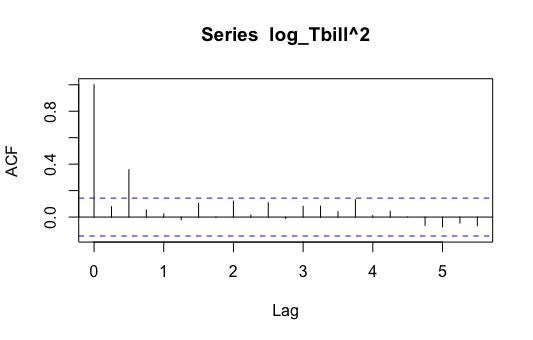
\includegraphics[width=0.4\linewidth]{logtbill2.png}
    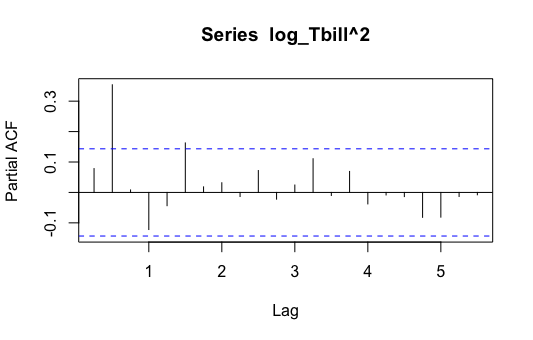
\includegraphics[width=0.4\linewidth]{pacflogtbill2.png}
\end{figure}
Observamos que los datos al cuadrado tienen un comportamiento similar a los anteriores, ambos decrecen a cero de manera rápida. Este hecho nos sugiere un modelo $GARCH(1,1)$ o similar. \\

Así pues, ajustamos a la serie un modelo $ARMA(0,1)/GARCH(1,1)$ y miramos si los coeficientes son significativos para comprobar si es un buen ajuste. 
\begin{table}[H]
\centering
\begin{tabular}{|
>{\columncolor[HTML]{EFEFEF}}c |c|c|}
\hline
\cellcolor[HTML]{C0C0C0}{\color[HTML]{000000} Parámetro} & \cellcolor[HTML]{C0C0C0}{\color[HTML]{000000} p-valor} & \cellcolor[HTML]{C0C0C0}{\color[HTML]{000000} Resultado} \\ \hline
$\hat{\mu}$                                              & $7.078042\cdot 10^{-3}$                                & Significativo                                            \\ \hline
$\hat{\phi}$                                             & $5.776659\cdot 10^{-5}$                                & Significativo                                            \\ \hline
$\hat{\omega}$                                           & $4.759324\cdot 10^{-2}$                                & Significativo                                            \\ \hline
$\hat{\alpha}$                                           & $2.672134\cdot 10^{-3}$                                & Significativo                                            \\ \hline
$\hat{\beta}$                                           & $2.433263\cdot 10^{-8}$                                & Significativo                                            \\ \hline
\end{tabular}
\end{table}
Dado que todos los valores anteriores son menores que el nivel de significancia impuesto, 0.05, rechazamos la hipótesis nula y aceptamos que los parámetros del modelo son estadísticamente significativos y por lo tanto, hemos ajustado nuestra serie a un buen modelo. \\


\section*{Ejercicio 2}
En el \textit{Black Monday} el rendimiento del S\&P 500 fue del -22,8\%, un gran fracaso. Queremos hacer un estudio sobre estos datos para intentar responder si este resultado era predecible o no. Así pues, empezaremos viendo cual era la probabilidad condicional de conseguir un rendimiento tan bajo usando datos de años anteriores. \\

Aqui podemos ver graficamente como bajó el rendimiento de una manera inusual:
\begin{figure}[H]
    \centering %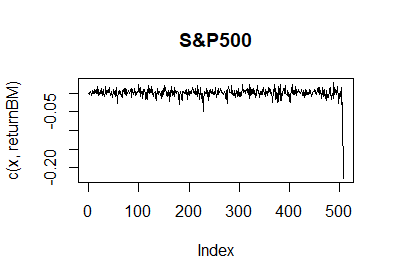
\includegraphics[width=0.5\linewidth]{Rplot01.png}
    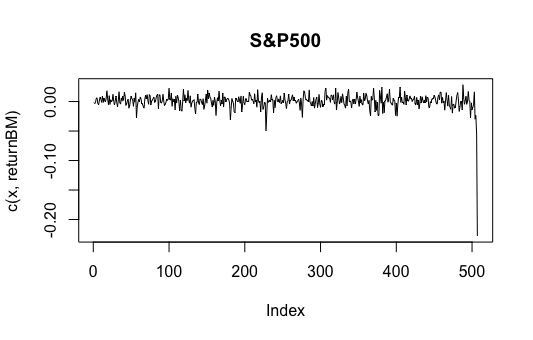
\includegraphics[width=0.5\linewidth]{sp.png}
\end{figure}


Para empezar, sabemos que a los dos ultimos años de datos antes del \textit{Black Monday} se les ajusta el modelo $AR(1)/GARCH(1,1)$. Recordemos que, dado $\{\varepsilon_{t}\}_t$ un $WN(0, \sigma_\epsilon^2)$, y las constantes $\alpha,\beta \geq 0,w >0,\mu $ y $\sigma $, definimos $\{Y_{t}\}_t$ como un proceso $AR(1)/GARCH(1,1)$ si

\begin{align*}
    Y_{t} - \mu &= \phi(Y_{t-1} - \mu) + a_{t} \\
    a_{t} &= \varepsilon_{t}\sigma_{t} \\
    \sigma_t&=\sqrt{w +\alpha a_{t-1}^2+\beta} \\
\end{align*}

Donde, $\{a_{t}\}$ corresponde a la parte de GARCH(1,1).\\

Calculamos ahora la probabilidad condicional de conseguir un rendimiento de -0.228 o menor que éste. Para hacerlo, utilizaremos los valores pasados: $Y_{k}$ para $k<t$ y las siguientes estimaciones para nuestras constantes: $\hat{\mu} = \bar{Y_{k}}$ , $ \hat{\phi}, \hat{\alpha}, \hat{\beta}, \hat{w} $. \\

Por lo tanto nos queda la siguiente formula   $Y_{t} - \hat{\mu} = \hat{\phi}(Y_{t-1} - \hat{\mu}) + a_{t} $ donde la única variable aleatoria es 
 $a_{t} = \varepsilon_{t}\sigma_{t}$. \\

Por lo que obtenemos la siguiente probabilidad:

\begin{align*}
    \mathbb{P}(Y_{t} \leq -0.228) &= \mathbb{P}(Y_{t} - \bar{Y_{t}} \leq -0.228 -\bar{Y_{t}}) = \mathbb{P}(a_{t} \leq -0.228 -\bar{Y_{t}})\\ &= \mathbb{P}(\varepsilon_{t}\sigma_{t}\leq -0.228 -\bar{Y_{t}}) = \mathbb{P}(\varepsilon_{t}\leq \frac{-0.228 -\bar{Y_{t}}}{\sigma_{t}})\\
\end{align*}

La distribución condicional del ruido blanco ($\varepsilon_{t}$) es la distribución t con un grado de libertad de $df$. Esto es, $\varepsilon_{t} \sim t_{df}.$ \\

Sustituyendo los estimadores por los valores que necesitamos obtenemos una probabilidad condicionada de $8.132691\cdot 10^{-5}$. Por lo que, el rendimiento del \textit{Black Monday} era impredecible con un modelo $AR(1)/GARCH(1,1)$. \\

Veamos como podemos mejorar nuestro modelo para que ajuste mejor nuestra serie, para ello analizaremos los residuos de $\{Y_{t}\}_t$. Primero calculamos los residuos estandalizados y los mostramos en el siguiente gráfico junto al gráfico ACF de éstos y de sus cuadrados.

\begin{figure}[H]
    \centering 
    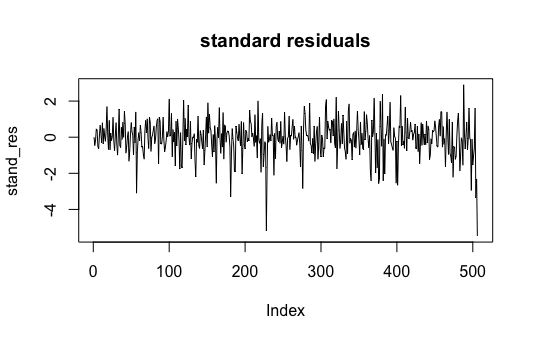
\includegraphics[width=0.5\linewidth]{stdres.png} 
\end{figure}

\begin{figure}[H]
    \centering
    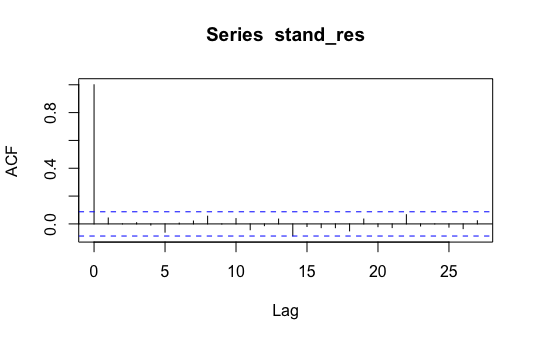
\includegraphics[width=0.4\linewidth]{stand_res.png}
    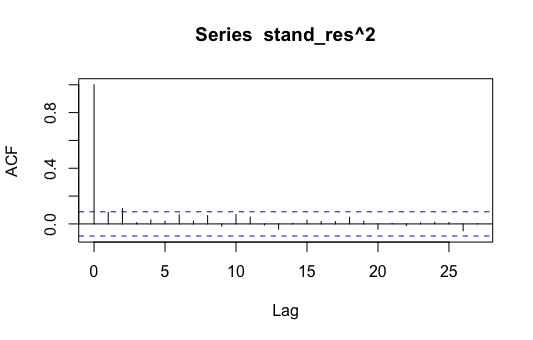
\includegraphics[width=0.4\linewidth]{stand_res^2.png}   
\end{figure}

Podemos ver en el gráfico de los residuos estandarizados que los residuos se dispersan alrededor de cero y nos hace pensar que el ruido se comporta como una distribución normal de $WN(0, \sigma_\epsilon^2)$ , ya que no tiene correlación porque después del \textit{lag} 0 todos los valores están dentro del rango de significancia cero. \\

Por lo que, podemos concluir que la parte $AR(1)$ del modelo es una buena adaptación de la serie temporal. Encontramos un comportamiento similar para el ACF de los residuos estandarizados al cuadrado. Vemos que todos los valores, después del \textit{lag} 0, están dentro del nivel de significancia. Eso indica que la parte $GARCH(1,1)$ del modelo tiene en cuenta la varianza condicional. \\

Analizamos ahora los gráficos ACF y PACF de los residuos sin estandarizar.
\begin{figure}[H]
    \centering 
    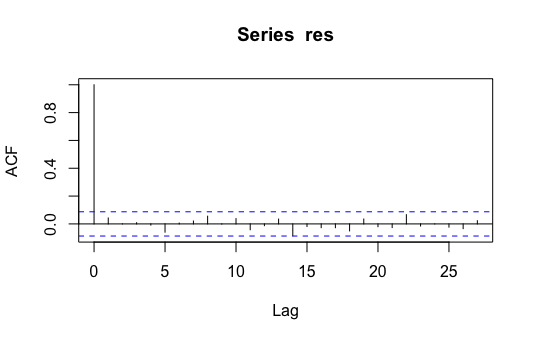
\includegraphics[width=0.4\linewidth]{acfres.png}
    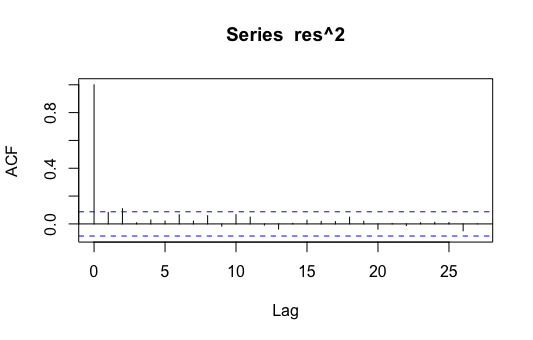
\includegraphics[width=0.4\linewidth]{acfres^2.png}
\end{figure}



En estos dos gráficos podemos ver que los residuos parecen no estar correlacionados, vemos que el ACF decae y después del \textit{lag} 0 todos los valores se encuentran dentro del rango de significancia cero. \\

Así pues, basándonos en los gráficos podemos pensar que el modelo parece encajar adecuadamente. \\

Para confirmar que el ajuste del modelo es bueno utilizaremos la prueba \textit{Ljung-Box}. Esta prueba tiene las siguientes hipótesis: la hipótesis nula nos dice que las correlaciones en la población de la que se toma la muestra son 0 y la hipótesis alternativa nos dice que los datos exhiben correlación serial. \\

Empezamos viendo la parte $AR(1)$:
\begin{lstlisting}[language=R]
> Box.test(res, type="Ljung")
	Box-Ljung test
p-value = 0.3358
\end{lstlisting}

Obtenemos que el p-valor es de 0,3358 y por lo tanto podemos aceptar la hipótesis nula de la prueba. Así pues vemos que $AR(1)$ sí que es un buen ajuste del modelo. \\


Veamos ahora si la parte $GARCH$ ajustada como $GARCH(1,1)$ es un buen modelo.

\begin{lstlisting}[language=R]
> Box.test(res^2, type="Ljung")
	Box-Ljung test
p-value = 0.06368
\end{lstlisting}

Con los residuos al cuadrado obtenemos un p-valor de 0,06368 que es mayor que 0,05. Por lo tanto, aceptamos la hipótesis nula y podemos decir que el ajuste encaja con el modelo. \\


Estudiamos ahora si podemos encontrar un modelo mejor para nuestra serie con otro $GARCH(P,Q)$. Por ejemplo, si hacemos el mismo estudio con $P=1$ y $Q=0$ tenemos el modelo $ARCH(1)$. ¿Es este mejor ajuste que el que teníamos? \\

Primero ajustamos los datos como un modelo $AR(1)/ARCH(1)$ y seguimos el mismo método que antes. Calculamos los residuos estandarizados y hacemos los gráficos ACF de éstos y de sus cuadrados.
\begin{figure}[H]
    \centering
    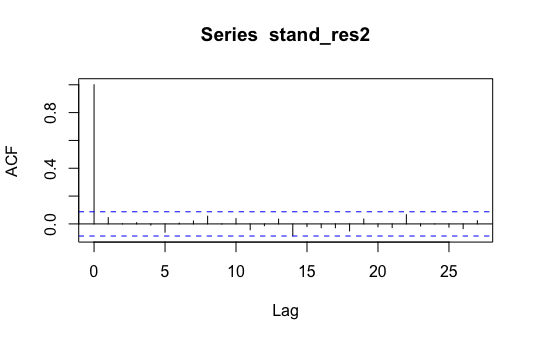
\includegraphics[width=0.4\linewidth]{stand_res2.png}
    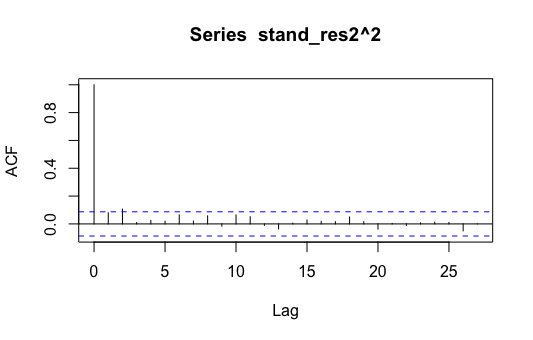
\includegraphics[width=0.4\linewidth]{stand_res2^2.png}  
\end{figure}

Vemos que con el modelo $AR(1)$ se consiguen unos resultados muy parecidos a los de antes, por lo que podemos suponer que sigue siendo una buena adaptación. En cambio, repitiendo el proceso anterior con los residuos estandarizados al cuadrado ahora vemos que los valores parecen ser ligeramente mayores que los del modelo anterior, lo que tal vez nos indique que este modelo se ajusta peor que el anterior. \\

Analizamos ahora los gráficos ACF y PACF de los residuos.

\begin{figure}[H]
    \centering
    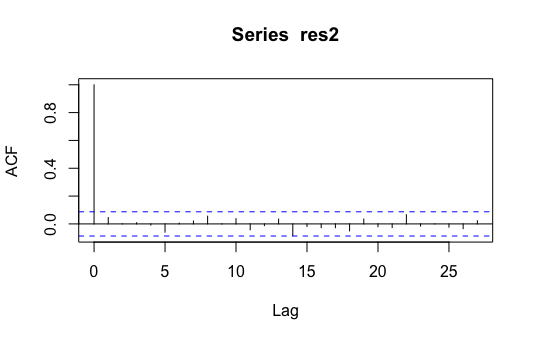
\includegraphics[width=0.4\linewidth]{res2.png}
    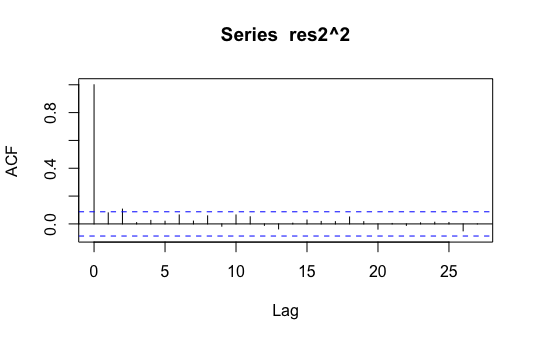
\includegraphics[width=0.4\linewidth]{res2^2.png}
\end{figure}

Podemos ver, de nuevo, que el ACF de los residuos se comporta de manera similar al anterior modelo. En cambio, el ACF de los residuos al cuadrado muestra un valor significativo distinto de cero para el segundo \textit{lag}, lo que sugiere que tal vez los residuos no sean independientes.
Por lo tanto podemos pensar que este modelo proporciona un peor ajuste que el anterior. \\

De nuevo, comprobamos como es el ajuste con una prueba \textit{Ljung-Box}.
\begin{lstlisting}[language=R]
> Box.test(res2, type="Ljung")
	Box-Ljung test
p-value = 0.3046
\end{lstlisting}
\begin{lstlisting}[language=R]
> Box.test(res2^2, type="Ljung")
	Box-Ljung test
p-value = 0.07339
\end{lstlisting}

Realizando esta prueba podemos ver un p-valor de 0,3046 y 0,0733 respectivamente. Así pues, dado que ambos valores son mayores que el nivel de significancia considerado, 0,05, no tenemos evidencia estadística suficiente para rechazar la hipótesis nula y aceptamos que los residuos no están correlacionados. Este hecho nos indica que el modelo parece encajar adecuadamente.\\


Por ultimo, veremos si un modelo AR(1) proporciona un ajuste adecuado del rendimiento de $S\&P500$.
En este caso, el ruido ya no sera una variable de GARCH. 
El proximo grafico nos enseña como es el ruido con este modelo, que sigue una distribución de $WN(0, \sigma_\epsilon^2)$

\begin{figure}[H]
    \centering 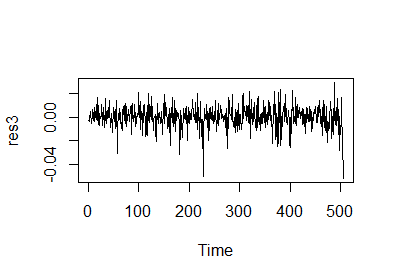
\includegraphics[width=0.4\linewidth]{Rplot08.png}
    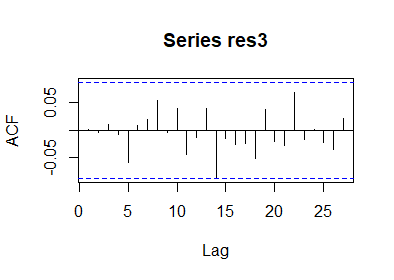
\includegraphics[width=0.4\linewidth]{Rplot09.png}
\end{figure}

Al analizar en ACF los residuos no muestran ninguna correlación visible entre sí, lo que significa simplemente
El modelo AR(1) encaja perfectamente.\\

Ademas, el test de \textit{Ljung-Box} nos da la misma información.
Obtenemos un p-valor de 0,9855 y por lo tanto nos quedamos con la hipótesis nula: los datos se distribuyen de forma independiente. De esta manera afirmamos que es un buen modelo.

\begin{figure}[H]
    \centering 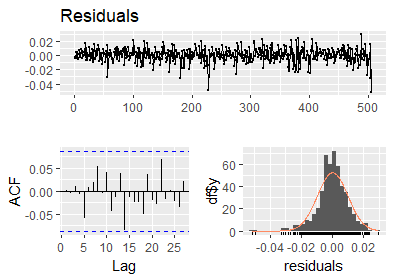
\includegraphics[width=0.5\linewidth]{Rplot10.png}
\end{figure}

\section*{Ejercicio 3}
Hemos reecibido un conjunto de datos y queremos elegir un modelo adecuado para éstos. Así pues, primero comencemos observando sus valores.
\begin{center}
    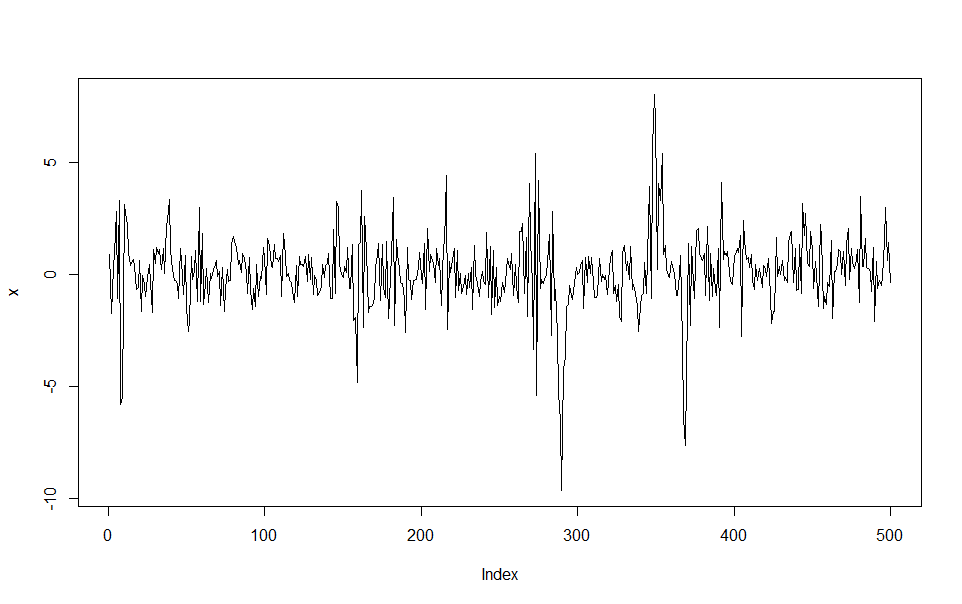
\includegraphics[width=0.7\linewidth]{DataHW2.png}
\end{center}

Vemos que la media es cercana a $0$ y experimentamos períodos de alta volatilidad y períodos de menor volatilidad.
Comenzando con el componente $ARMA(p, q)$, consideremos trazar el ACF y PACF, para obtener los parámetros p y q:

\begin{figure}[H]
    \centering 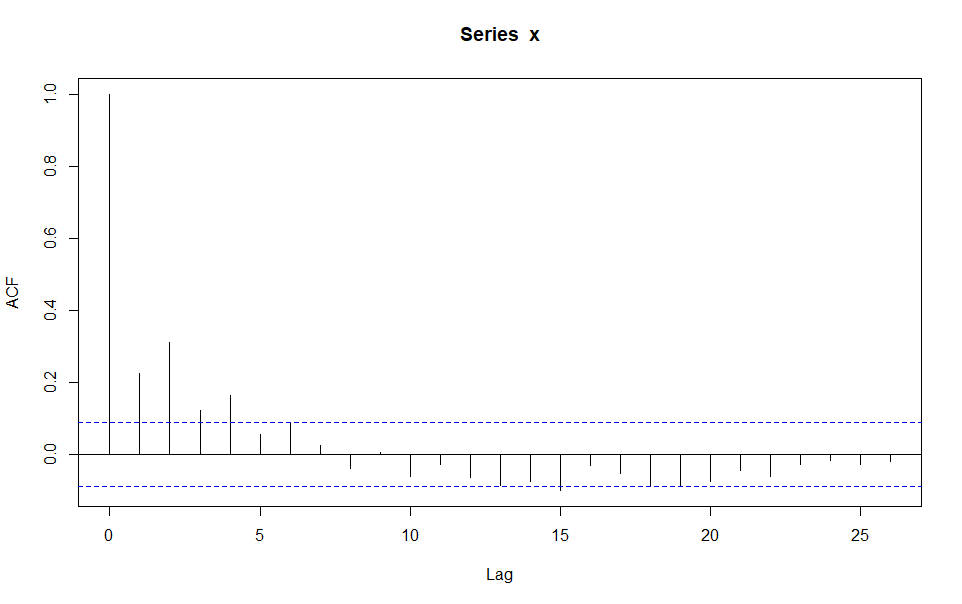
\includegraphics[width=0.49\linewidth]{ACF-HW2.png}
    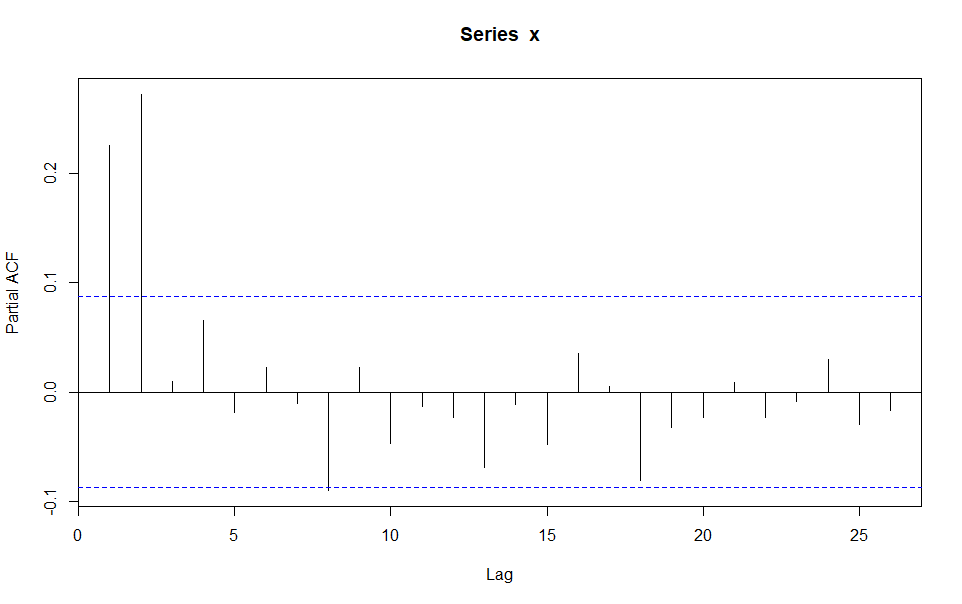
\includegraphics[width=0.49\linewidth]{PACF-HW2.png}
\end{figure}

Con estos gráficos podemos ver claramente que es muy probable que el parámetro relacionado con $MA$ sea 0, y el
otro cerca de 2. Esto cumple con la sugerencia que obtuvimos, q = 0. Para obtener el modelo completo y obtener información
Sobre la componente GARCH(P, Q), procedamos el estudio con los gráficos de los cuadrados:

\begin{figure}[H]
    \centering 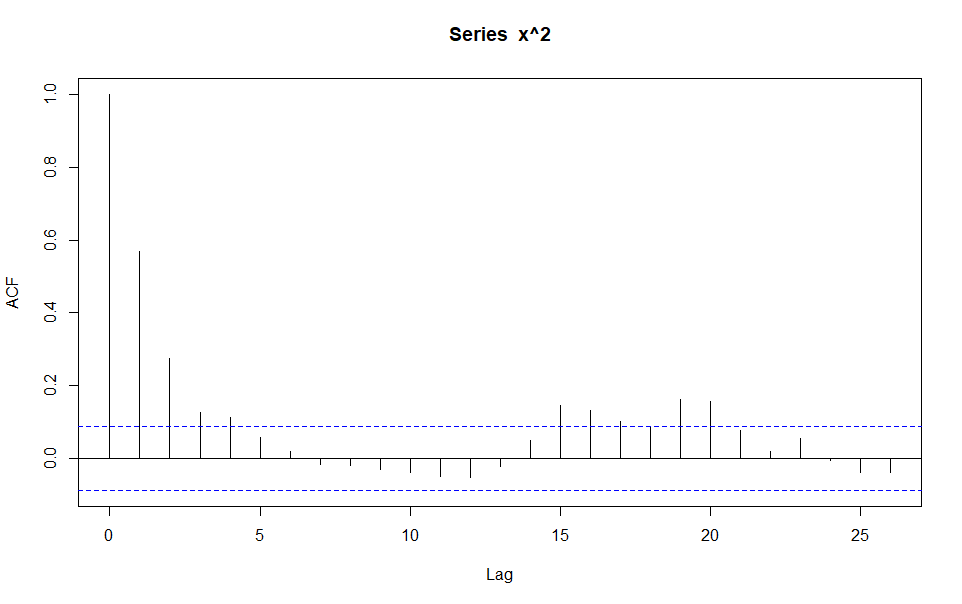
\includegraphics[width=0.49\linewidth]{ACFX^2.png}
    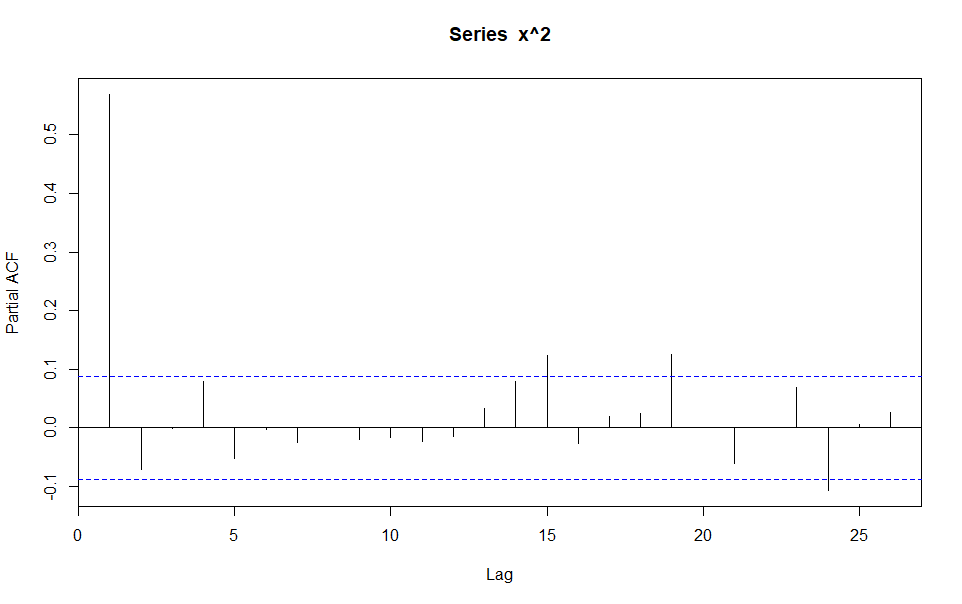
\includegraphics[width=0.49\linewidth]{PACFX^2.png}
\end{figure}

Teniendo esto en cuenta, un parámetro será 0 y el otro 1 o 2.
Después de probar algunas combinaciones y usar el criterio AICC para elegir, decidimos seguir con ARMA(2, 0) y
GARCH(1, 0). Obtenemos todos los valores que son significativos. Con este ajuste del modelo, comprobar el comportamiento de los residuos necesario requiere para demostrar que se ajusta perfectamente y es útil para las predicciones. Veamos los gráficos ACF y PACF de los
residuos y sus cuadrados:

\begin{figure}[H]
    \centering 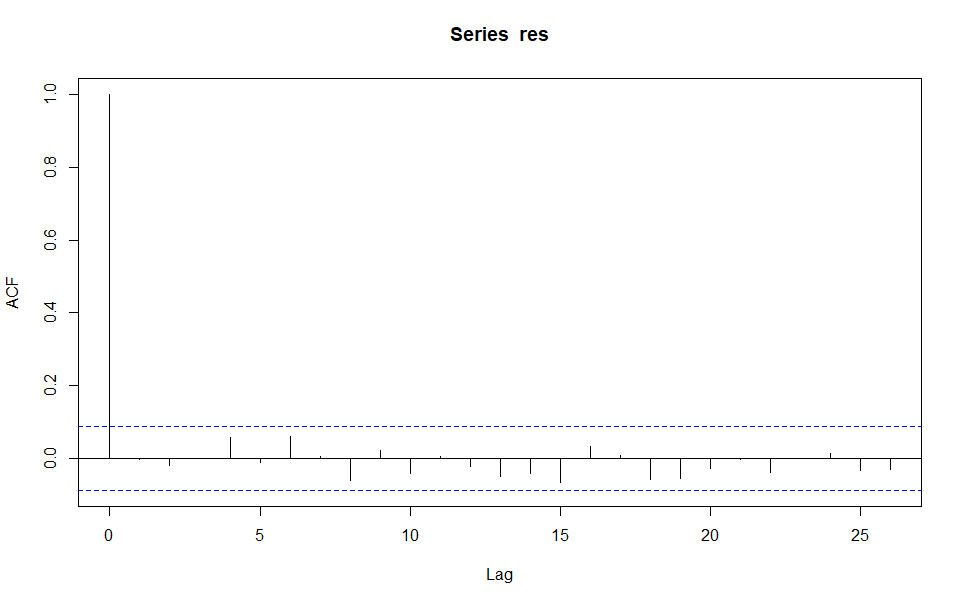
\includegraphics[width=0.49\linewidth]{Res-ACF.png}
    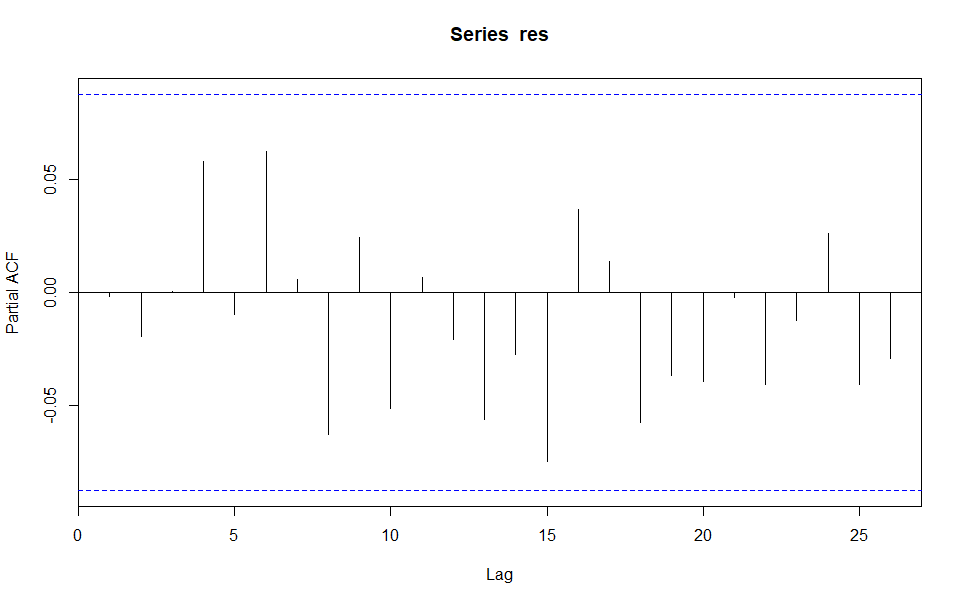
\includegraphics[width=0.49\linewidth]{Res-PACF.png}
\end{figure}

Al realitzar el test, nos damos cuenta que el el p-valor es mayor que el nivel de significancia, por lo tanto no estan correlacionados. Por lo tanto, podemos decir que ARMA(2,0) ajusta bien el modelo. Para estudiar ahora el modelo ARMA(2,0)/GARCH(P,Q), tenemos que encontrar qué P y Q hacen que el modelo elegido tenga un buen ajuste. Para eso representamos la serie temporal de los residuos al cuadrado.

\begin{figure}[H]
    \centering 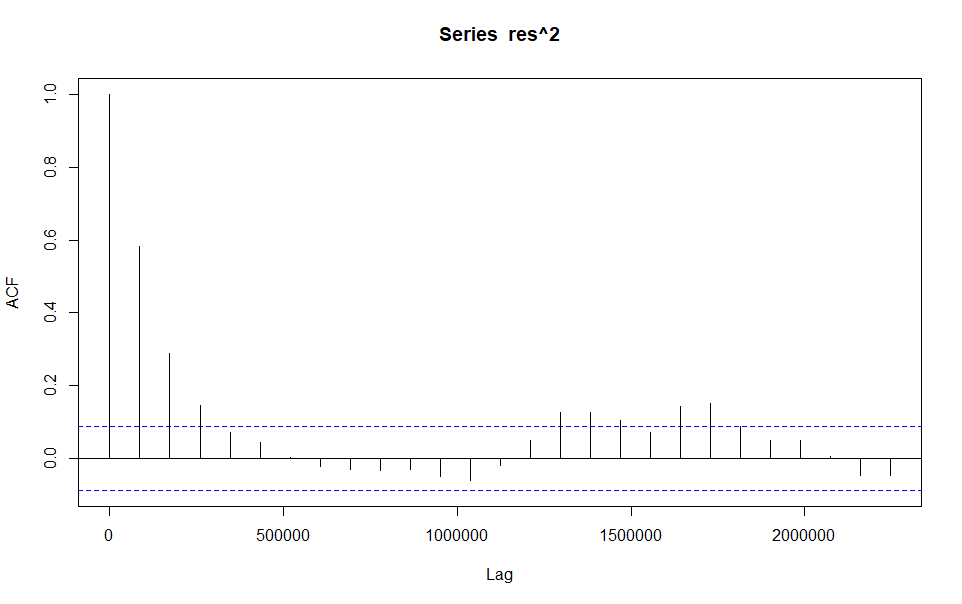
\includegraphics[width=0.49\linewidth]{ACF-Res^2.png}
    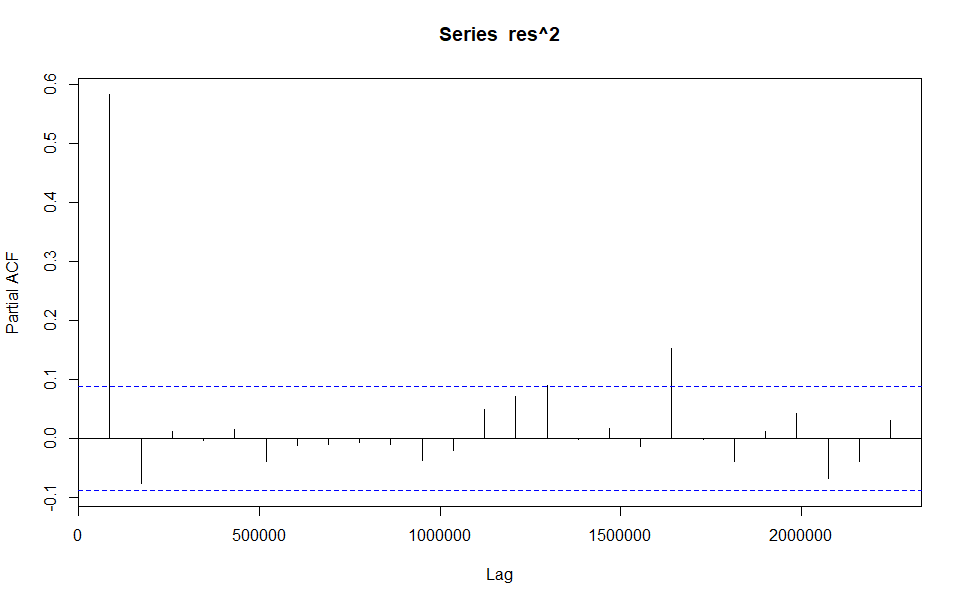
\includegraphics[width=0.49\linewidth]{PACF-Res^2.png}
\end{figure}

Podemos ver que parece que siga un modelo GARCH(1,0) ya que hay un fuerte descenso en el gráfico PACF (p=1) y un descenso muy lento en el gráfico ACF (q=0). Tras provar los diferentes valores para P y Q (entre 0 y 2) y realizar los respectivos tests de AIC i BIC nos damos cuenta que el modelo que nos ofrece menor AIC y BIC es un modelo GARCH(1,0), con un AIC de $3.161444$ y un BIC de $3.203590$.

\begin{table}[]
\centering
\begin{tabular}{|l|l|l|}
\hline
                     & AIC      & BIC      \\ \hline
ARMA(2,0)/GARCH(1,0) & 3.161444 & 3.203590 \\ \hline
ARMA(2,0)/GARCH(1,1) & 3.165406 & 3.215982 \\ \hline
ARMA(2,0)/GARCH(1,2) & 3.172969 & 3.231974 \\ \hline
ARMA(2,0)/GARCH(2,0) & 3.168999 & 3.219575 \\ \hline
ARMA(2,0)/GARCH(2,1) & 3.172999 & 3.232004 \\ \hline
ARMA(2,0)/GARCH(2,2) & 3.176969 & 3.244403 \\ \hline
\end{tabular}
\end{table}

Estos son los valores obtenidos a partir de los diferentes modelos. Ahora, necesitamos ajustar un modelo GARCH a nuestros datos y estimar los parámetros del modelo. Por lo cual nos facilita el análisis y la gestión de la volatilidad en las series temporales financieras. Para ello usaremos la función ugarchspec. Volviendo a mirar el AIC i BIC de dichos modelos vemos que el modelo que tiene tanto el AIC como el BIC más bajo es el ARMA(2,0)/GARCH(1,0). Finalmente comprobamos que todos los coeficientes son significativos mirando los residuos y su ACF y PACF.

\begin{figure}[H]
    \centering 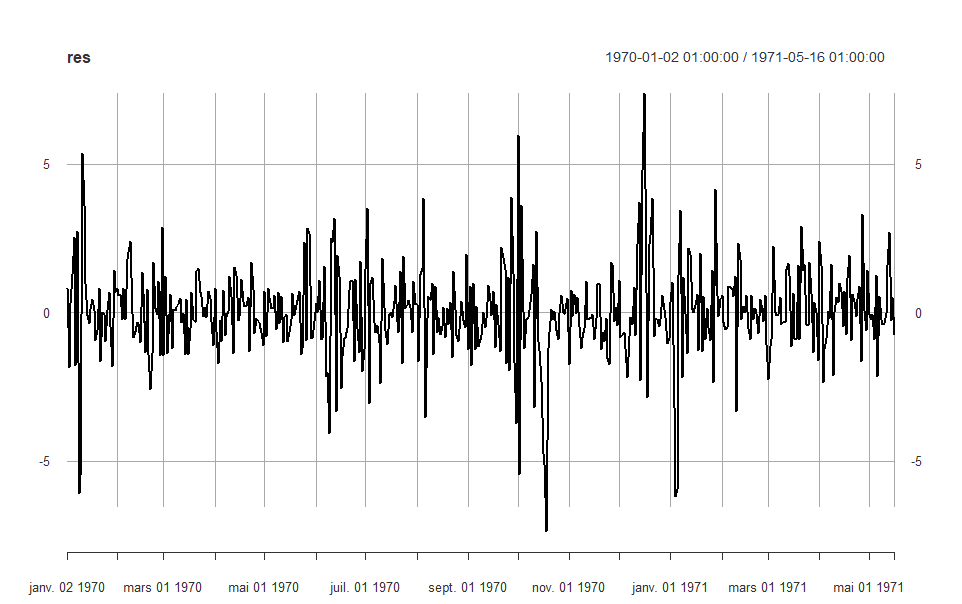
\includegraphics[width=0.49\linewidth]{Res.png}
\end{figure}

\begin{figure}[H]
    \centering 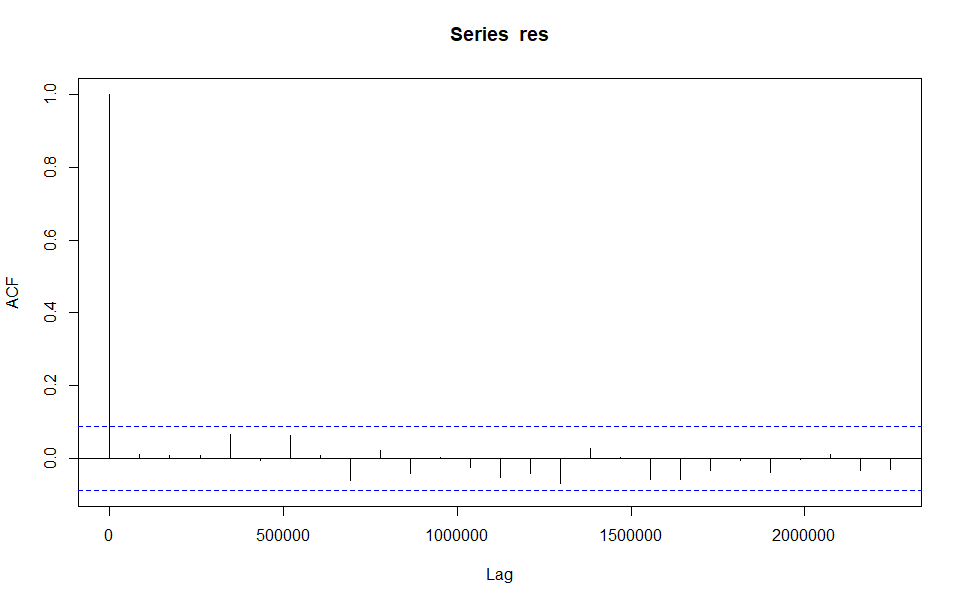
\includegraphics[width=0.49\linewidth]{glkn.png}
\end{figure}

\begin{figure}[H]
    \centering 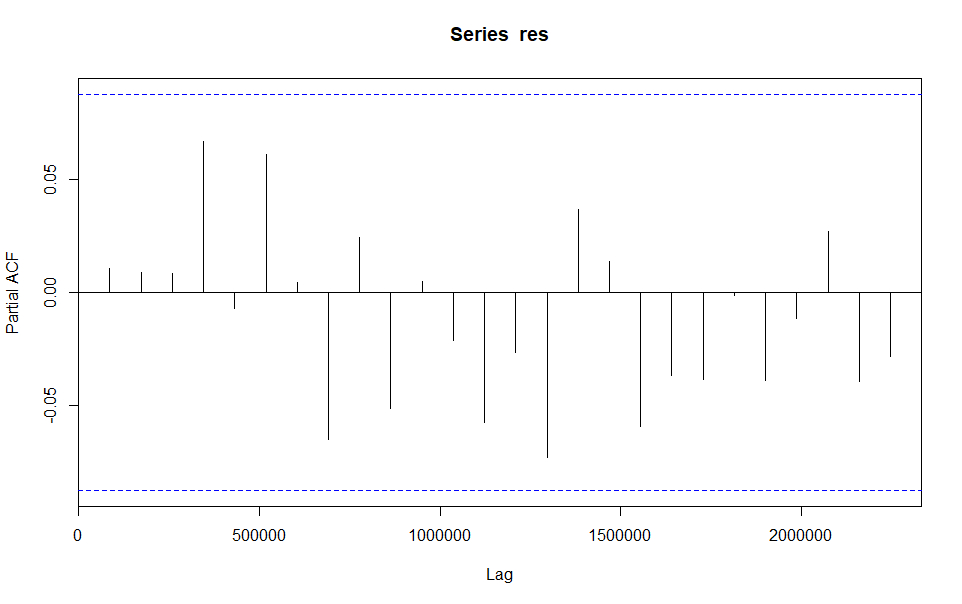
\includegraphics[width=0.49\linewidth]{ref.png}
\end{figure}

Vemos que los residuos no estan correlacionados, lo que nos indica que es un buen modelo. 

\end{document}